% !TeX spellcheck = en_US
\section{Molecular bonding}
The two principal types of bonds are the ionic and the covalent bond. 
Other types of bonds are van der Waals bonds, metallic bonds and hydrogen bonds.

Balance between attractive force $E_A$ (e.g. Coulomb force) and repulsive force $E_R$ (shell overlap).

\begin{figure}[ht]
    \centering
    \begin{tikzpicture}
\pgfplotsset{ticks=none}
\pgfplotsset{every axis x label/.style={
    at={(0.5,0)},
    below,
    yshift=-5pt}
}
\pgfplotsset{every axis y label/.style={
    at={(0,0.5)},
    xshift=-15pt,
    rotate=90}
}

\begin{scope}[shift={(-5,0)}]
    \begin{axis}[domain=0.05:1,samples=101,
        width = 8cm, height = 6cm,
        xlabel={Interatomic separation $r$},
        ylabel={Force},
        xmin = 0.1, xmax = 0.5,
        ymin = -1000, ymax = 1000,
    ]
        \addplot[black!80,mark=none] coordinates {(0,0)(1,0)};
        \node at (axis cs:0.11,65) {0};
        \addplot[HSRBlue,mark=none] {20/(x^2)};
        \addplot[HSRBlue,mark=none] {-0.25/(x+0.1)^6};
        \addplot[HSRHematite,mark=none] {20/(x^2) - 0.25/(x+0.1)^6};
        \node[label={$r_0$},circle,fill=HSRHematite,inner sep=2pt] at (axis cs:0.16334,1) {};
        \node at (axis cs:0.25,500) {$F_A$};
        \node at (axis cs:0.21,-500) {$F_R$};
        \node at (axis cs:0.25,65) {$F_N$};
    \end{axis}
\end{scope}

\begin{scope}[shift={(+5,0)}]
    \begin{axis}[domain=0:1,samples=101,
        width = 8cm, height = 6cm,
        xlabel={Interatomic separation $r$},
        ylabel={Potential Energy},
        xmin = 0, xmax = 0.8,
        ymin = -200, ymax = 100,
    ]
        \addplot[black!80,mark=none] coordinates {(0,0)(1,0)};
        \node at (axis cs:0.02,15) {0};
        \addplot[HSRBlue,mark=none] {-20/x};
        \addplot[domain=0.11:1,HSRBlue,mark=none] {1/(20*(x+0.1)^5)};
        \addplot[HSRHematite,mark=none] {1/(20*(x+0.1)^5) - 20/x};
        \node[label={ $r_0$},circle,fill=HSRHematite,inner sep=2pt] at (axis cs:0.16334,-82.96) {};
        \node at (axis cs:0.4,20) {$E_R$};
        \node at (axis cs:0.4,-70) {$E_A$};
        \node at (axis cs:0.4,-30) {$E$};
    \end{axis}
\end{scope}


\end{tikzpicture}
    \caption{Force and energy in molecular bonding}
\end{figure}

where $r_0$ is the equilibrium separation and $E_0$ the bond energy at equilibrium.

\subsection{Ionic bonding}
%TODO: add images / example

\begin{equation}
	E(r) = -\frac{e^2 M}{\varepsilon_0 4 \pi r} + \frac{B}{r^m}
\end{equation}
where $M$, $B$ and $m$ are constants. 

$M$ is the Mandelung constant, which models Coulomb interactions in the ionic crystal.
It depends on the crystal type and is $M=1.748$ for a \ce{NaCl} type (FCC).
For NaCl crystal, $B=\SI{6.972e-96}{\joule\meter\tothe{8}}$ and $m=8$.

\subsection{Covalent bonding} 
Atoms share electrons to fill their valence bands.

\subsection{Metallic bonding}
Atoms are held together by electron gas.

\subsection{Secondary (Van der Waals) bonding}
Weak force between polar molecules (dipoles, e.g. \ce{H2O}). 

\subsection{Comparison} ~\\
\begin{table}[ht]
    \begin{tabularx}{\linewidth}{p{2cm}p{1.5cm}p{1.4cm}p{1.4cm}p{1.5cm}lX}
    	& Typical Solids & Bond Energy  & Melt. Temp. & Elastic Modulus & Density & Typical Properties \\ \toprule
    	Ionic & NaCl & 3.2 & 801 & 40 & 2.17 & El. insulators (may become conductive at high temperatures). \\
    	 & MgO & 10 & 2852 & 250 & 3.58 & High elastic modulus. Hard and brittle but cleavable. Th. conductivity less than metals.\\
    	Metallic & Cu & 3.1 & 1083 & 120 & 8.96 & El. conductor. \\
    	 & Mg & 1.1 & 650 & 44 & 1.74 & Good th. conduction. High elastic modulus. Generally ductile, can be shaped. \\
    	Covalent & Si & 4 & 1410 & 190 & 2.33 & Large elastic modulus, hard and brittle. \\
    	  & C & 7.4 & 3550 & 827 & 3.52 & Diamond. Hardest material, good el. insulator. \\
    	van der Waals: Hydrogen & PVC & - & 212 & 4 & 1.3 & Low elastic modulus. Some ductility \\
    	 & H$_2$O (ice) & 0.52 & 0 & 9.1 & 0.917 & El. insulator, poor th. conductivity, large thermal expansion. \\
        van der Waals: Induced dipole & Crystalline Argon & 0.09 & -189 & 8 & 1.8 & Low elastic modulus, el. insulator, poor th. conductivity, large th. expansion. \\
    	\bottomrule
    \end{tabularx}
    \caption{Comparison of bond types and typical properties}
\end{table}

\subsection{Crystal structures}

The atomic packaging factor $\mathrm{APF}$ is defined as
\begin{equation}
    \mathrm{APF} = \frac{\text{Volume of atoms in unit cell}}{\text{Volume of unit cell}}
\end{equation}

\begin{figure}[ht!]
    \centering
    \begin{subfigure}[t]{0.32\linewidth}
        \centering
        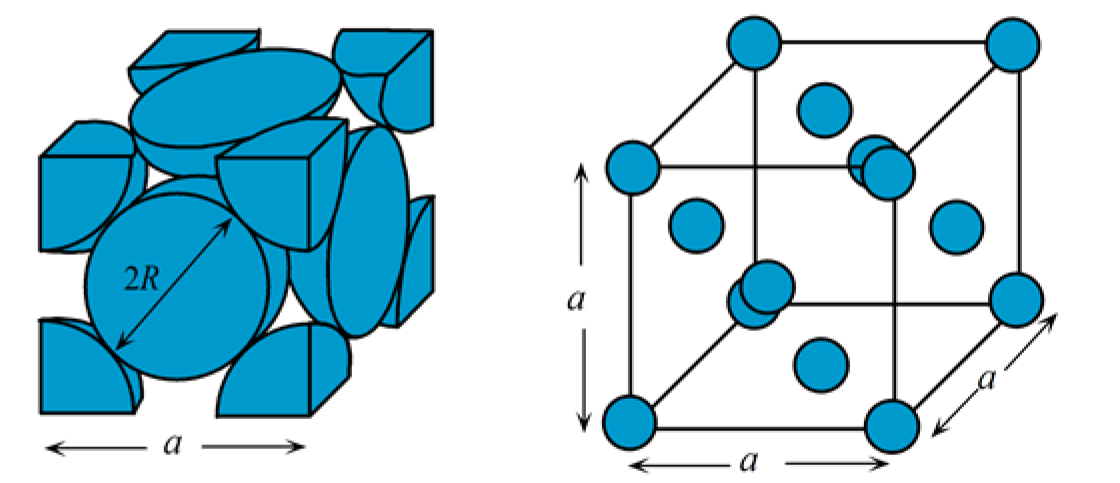
\includegraphics[width=0.9\textwidth]{images/fcc.png}
        \caption{Face-centered cubic (FCC)}
    \end{subfigure}
    \begin{subfigure}[t]{0.32\linewidth}
        \centering
        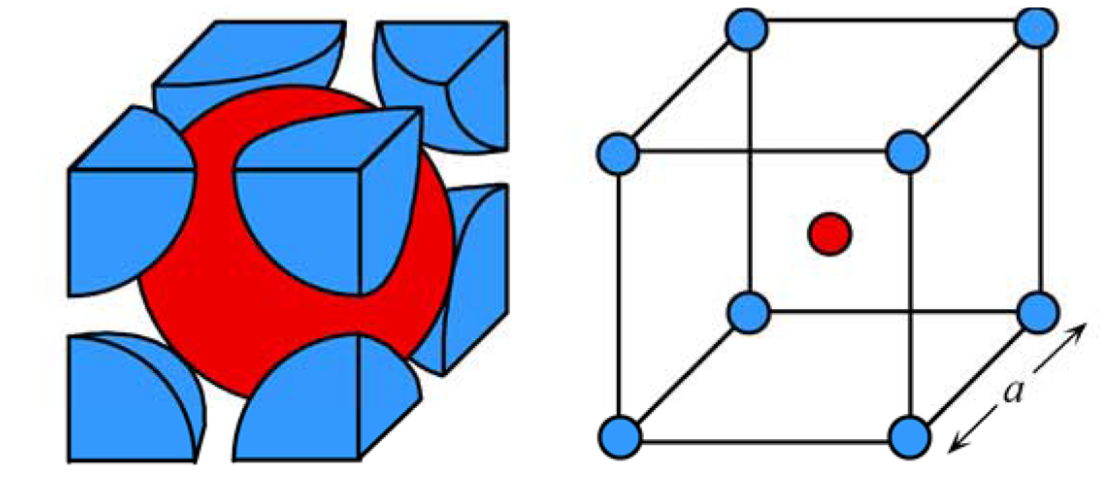
\includegraphics[width=0.9\textwidth]{images/bcc.png}
        \caption{Body-centered cubic (BCC)}
    \end{subfigure}
    \begin{subfigure}[t]{0.32\linewidth}
        \centering
        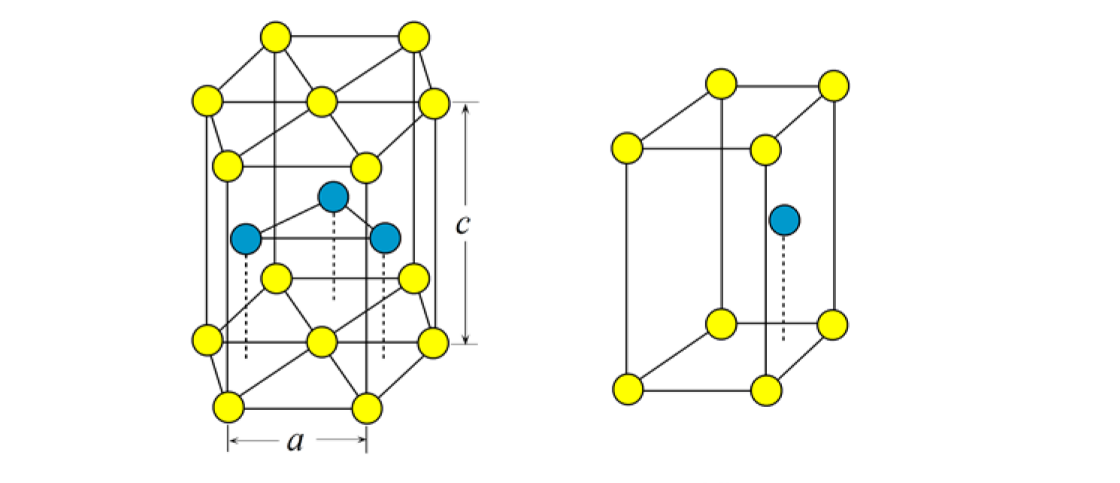
\includegraphics[width=0.9\textwidth]{images/hcp.png}
        \caption{Hexagonal close-packed (HCP)}
    \end{subfigure} 
    
    \begin{subfigure}[t]{0.24\linewidth}
        \centering
        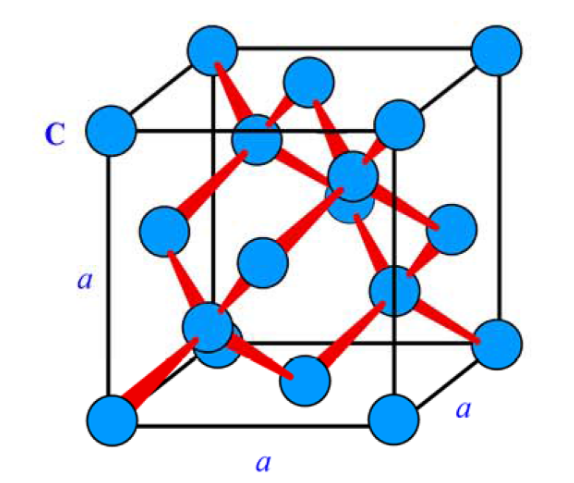
\includegraphics[width=0.9\textwidth]{images/diamond.png}
        \caption{Diamond unit cell}
    \end{subfigure}
    \begin{subfigure}[t]{0.24\linewidth}
        \centering
        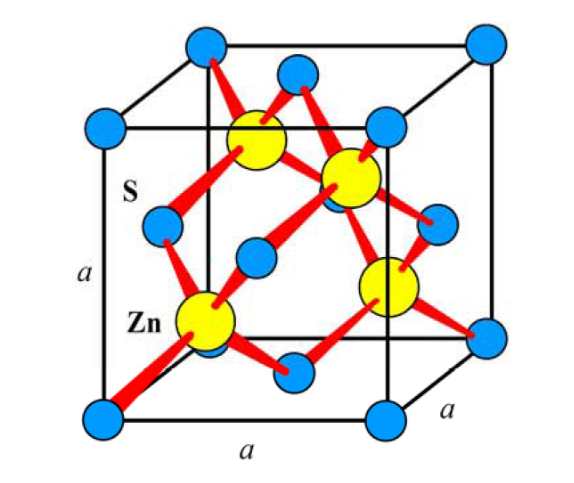
\includegraphics[width=0.9\textwidth]{images/zns.png}
        \caption{Zinc blende (ZnS) cubic structure}
    \end{subfigure} 
    \begin{subfigure}[t]{0.24\linewidth}
        \centering
        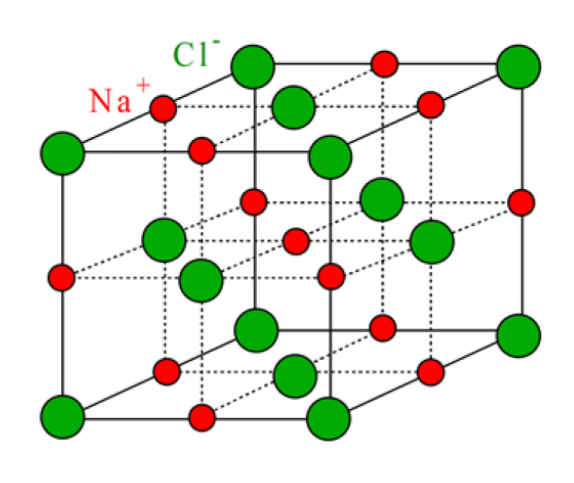
\includegraphics[width=0.9\textwidth]{images/nacl.png}
        \caption{Ionic NaCl crystal structure}
    \end{subfigure}  
    \begin{subfigure}[t]{0.24\linewidth}
        \centering
        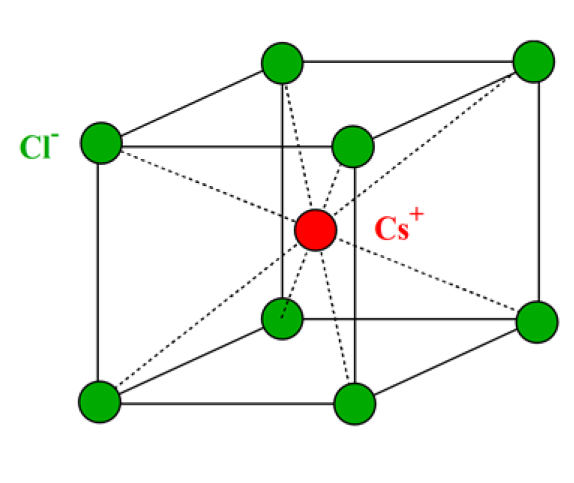
\includegraphics[width=0.9\textwidth]{images/cscl.png}
        \caption{Ionic CsCl crystal structure}
    \end{subfigure}     
    \caption{Comparison of unit cells}
\end{figure}

\begin{table}[ht!]
    \centering
    \begin{tabularx}{0.9\linewidth}{p{2cm}p{2cm}p{2.5cm}p{1.8cm}p{1.5cm}X}
    \toprule
        Crystal Structure & $a$ and $R$ & Coordination Number (CN) & Atoms per unit cell & APF & Examples \\ \midrule
        Simple cubic & $a = 2R$ & 6 & 1 & 0.52 & None \\
        BCC & $a=4R/\sqrt{3}$ & 8 & 2 & 0.68 & Metals: $\alpha-$Fe, Cr,Mo,W \\
        FCC & $a=4R/\sqrt{2}$ & 12 & 4 & 0.74 & Metals: Ag, Au, Cu, Pt \\
        HCP & $a=2R$, $c=1.633a$ & 12 & 2 & 0.74 & Metals: Co, Mg, Ti, Zn \\
        Diamond & $a=8R/\sqrt{3}$ & 4 & 8 & 0.34 & Covalent solids: Diamond, Ge, Si, $\alpha-$Sn \\
        ZnS & & 4 & 8 & 0.34 & Covalent and ionic solids, compound semiconductors: ZnS, GaAs, GaSb, InAs, InSb \\
        NaCl & & 6 & 4 cations, 4 anions & 0.67 & Ionic solids: NaCl, AgCl, LiF, MgO, CaO \\
        CsCl & & 8 & 1 cation, \newline 1 anion & & Ionic solids: CsCl, CsBr, CsI \\
    \bottomrule
    \end{tabularx}
    \caption{Properties of some important crystal structures}
\end{table}

\subsection{Allotropy and carbon}
Certain substances can have more than one crystal structure. 
E.g. carbon has eight allotropes: Diamond, Graphite, Lonsdaleite, $C_{60}$ (buckyball), $C_{540}$, $C_{70}$, amorphous carbon and single-walled carbon nanotube.